% This is part of Un soupçon de mathématique sans être agressif pour autant
% Copyright (c) 2012-2013
%   Laurent Claessens
% See the file fdl-1.3.txt for copying conditions.

\EpsOrPdfincludegraphics[width=\linewidth]{BO_perspective}

\begin{example}
    Dessiner un cube comme vous le voulez en suivant le quadrillage de la feuille. Quelle est la longueur des arrêtes en profondeur ? Avec quel angle vous les dessinez ?
\end{example}

%+++++++++++++++++++++++++++++++++++++++++++++++++++++++++++++++++++++++++++++++++++++++++++++++++++++++++++++++++++++++++++
\section{Droites et plans dans l'espace}
%+++++++++++++++++++++++++++++++++++++++++++++++++++++++++++++++++++++++++++++++++++++++++++++++++++++++++++++++++++++++++++

%--------------------------------------------------------------------------------------------------------------------------- 
\subsection{Introduction}
%---------------------------------------------------------------------------------------------------------------------------

La figure \ref{LabelFigDesSections} montre un cube. Êtes-vous capables de donner la nature des surfaces coloriées ?
\newcommand{\CaptionFigDesSections}{Exercice de vision dans l'espace.}
\input{Fig_DesSections.pstricks}
Le triangle vert est isocèle et rectangle parce que deux de ses côtés sont des arrêtes du cube. Le triangle rouge est plus troublant, mais il est équilatéral : ses trois côtés sont des diagonales des faces du cube. Notez que \emph{sur le dessin}, les trois côtés ont des longueur différentes.


%---------------------------------------------------------------------------------------------------------------------------
\subsection{Deux droites}
%---------------------------------------------------------------------------------------------------------------------------

\begin{Aretenir}
    \begin{enumerate}
        \item
            Dans un plan, il existe une et une seule droite parallèle à une droite donnée passant par un point donné.
        \item
            Cette propriété est encore valable dans l'espace.            
    \end{enumerate}
\end{Aretenir}

Deux droites peuvent être soit dans un même plan, soit ne pas être dans le même plan. Deux droites contenues dans un même plan sont dires \defe{coplanaires}{coplanaire}.
\begin{multicols}{2}
    \begin{center}
        Droites coplanaires
    \end{center}
\begin{Aretenir}
    Si deux droites sont contenues dans un même plan, alors soit elles sont parallèles, soit elles sont sécantes. 
\end{Aretenir}

    \columnbreak

    \begin{center}
        Droites non coplanaires.
    \end{center}
\begin{Aretenir}
    Deux droites non coplanaires ne sont ni sécantes ni parallèles.
\end{Aretenir}

\end{multicols}

Des exemples sont donnés à la figure \ref{LabelFigPositionsDroitesbnYIsH}. % From file PositionsDroitesbnYIsH
\newcommand{\CaptionFigPositionsDroitesbnYIsH}{Droites coplanaires ou non.}
\input{Fig_PositionsDroitesbnYIsH.pstricks}

%See also the subfigure \ref{LabelFigPositionsDroitesbnYIsHssLabelSubFigPositionsDroitesbnYIsH0}
%See also the subfigure \ref{LabelFigPositionsDroitesbnYIsHssLabelSubFigPositionsDroitesbnYIsH1}
%See also the subfigure \ref{LabelFigPositionsDroitesbnYIsHssLabelSubFigPositionsDroitesbnYIsH2}
Notez en particulier la figure \ref{LabelFigPositionsDroitesbnYIsHssLabelSubFigPositionsDroitesbnYIsH3} sur laquelle les droites \( (FH)\) et \( (AC)\) ne sont pas sécantes !

\begin{propriete}
    Deux droites sécantes sont toujours coplanaires.
\end{propriete}

\begin{proof}
    Soient \( d\) et \( d'\) deux droites sécantes dans l'espace. Soit \( K\) leur point d'intersection; soit \( A\), un autre point sur \( d\) et \( B\) un autre point sur \( d'\).

    Le plan défini par les points \( A\), \( K\) et \( B\) contient les deux droites.
\end{proof}

%---------------------------------------------------------------------------------------------------------------------------
\subsection{Deux plans}
%---------------------------------------------------------------------------------------------------------------------------

\begin{definition}
    Deux plans sont \defe{parallèles}{parallèle!deux plans} soit si ils sont confondus, soit si ils n'ont aucun point commun.
\end{definition}


Deux plans dans l'espace sont soit parallèles, soit sécants.
\begin{multicols}{2}

    \begin{center}
        Plans parallèles
    \end{center}
    Des plans parallèles sont soit confondus, soit n'ont aucun point communs.

Les plans \( (AEB)\) et \( (DHC)\) ci-contre sont parallèles.

\columnbreak

%The result is on figure \ref{LabelFigPositionPlansTvKvah}. % From file PositionPlansTvKvah
%\newcommand{\CaptionFigPositionPlansTvKvah}{<+Type your caption here+>}
    \begin{center}
\input{Fig_PositionPlansTvKvah.pstricks}
    \end{center}


\end{multicols}

\begin{multicols}{2}
    \begin{center}
        Plans sécants
    \end{center}
    L'intersection de deux plans sécants (non confondus) est une droite.

    L'intersection des plans \( (ABG)\) et \( (DCG)\) ci-contre est la droite \( (HG)\).

    \columnbreak

%The result is on figure \ref{LabelFigPositionPlansqSltxa}. % From file PositionPlansqSltxa
%\newcommand{\CaptionFigPositionPlansqSltxa}{<+Type your caption here+>}
    \begin{center}
\input{Fig_PositionPlansqSltxa.pstricks}
    \end{center}

\end{multicols}

%---------------------------------------------------------------------------------------------------------------------------
\subsection{Une droite et un plan}
%---------------------------------------------------------------------------------------------------------------------------

\begin{definition}
    Une droite est \defe{parallèle}{parallèle!droite et plan} à un plan lorsque soit la droite est contenue dans le plan, soit elle n'a aucun point commun avec le plan.
\end{definition}

\begin{multicols}{2}

    \begin{center}
        Droite et plan sécants
    \end{center}

    La droite \( (FD)\) intersecte le plan \( (ABH)\) au point \( M\).
%he result is on figure \ref{LabelFigfigureBCtCTZo}. % From file figureBCtCTZo
%\newcommand{\CaptionFigfigureBCtCTZo}{<+Type your caption here+>}

    \columnbreak
    \begin{center}
\input{Fig_figureBCtCTZo.pstricks}
    \end{center}
\end{multicols}

\begin{multicols}{2}

    \begin{center}
        Droite et plan parallèles
    \end{center}

    La droite \( (HC)\) et le plan \( (EBF)\) sont parallèles.

    \columnbreak
    \begin{center}
%The result is on figure \ref{LabelFigfigureASkECWS}. % From file figureASkECWS
%\newcommand{\CaptionFigfigureASkECWS}{<+Type your caption here+>}
\input{Fig_figureASkECWS.pstricks}
    \end{center}
\end{multicols}

\begin{multicols}{2}

    \begin{center}
        Droite contenue dans un plan
    \end{center}

    La droite \( (EB)\) est contenue dans le plan \( (AEF)\).

    \columnbreak
    \begin{center}
%The result is on figure \ref{LabelFigfigureCSIQETx}. % From file figureCSIQETx
%\newcommand{\CaptionFigfigureCSIQETx}{<+Type your caption here+>}
\input{Fig_figureCSIQETx.pstricks}
    \end{center}
\end{multicols}

\begin{definition}
    Une droite est \defe{perpendiculaire}{perpendiculaire!droite et plan} à un plan si elle est perpendiculaire à deux droites non confondues du plan.
\end{definition}

\begin{Aretenir}
    Si la droite \( d\) est perpendiculaire au plan \( \Omega\), alors toutes les droites du plan \( \Omega\) sécantes avec \( d\) sont perpendiculaires à \( d\).
\end{Aretenir}

\begin{remark}
    Seules deux droites peuvent être ni parallèle ni sécantes.
\end{remark}

%+++++++++++++++++++++++++++++++++++++++++++++++++++++++++++++++++++++++++++++++++++++++++++++++++++++++++++++++++++++++++++
\section{Les règles de la perspective cavalière}
%+++++++++++++++++++++++++++++++++++++++++++++++++++++++++++++++++++++++++++++++++++++++++++++++++++++++++++++++++++++++++++

Lorsque nous dessinons en trois dimension, nous prenons les conventions suivantes qui définissent la \defe{\wikipedia{fr}{Perspective_cavalière}{perspective cavalière}}{perspective!cavalière}.

\begin{Aretenir}
    D'abord nous choisissons
    \begin{enumerate}
        \item
            Nous choisissons un \defe{angle de fuite}{angle!de fuite} \( \alpha\) qui sera entre \unit{30}{\degree} et \( \unit{45}{\degree}\) avec l'horizontale\footnote{Sur une feuille à carreaux, le plus simple est de prendre \unit{45}{\degree}.}.
        \item
            Un \defe{coefficient de réduction}{coefficient de réduction} que nous noterons \( k\) et qui sera compris entre \( 0\) et \( 1\).
    \end{enumerate}

    Ensuite nous prenons les correspondances suivantes entre la réalité et le dessin :
    \begin{center}
        \begin{tabular}{|p{7.5cm}|p{7.5cm}|}
            \hline
            {\bf dans la réalité}&{\bf sur le dessin}\\
            \hline\hline
            Segment caché  & Segment pointillé\\
            \hline
            Segment parallèle à la feuille de dessin & Segment représenté en vraie grandeur\\
            \hline
            Segment perpendiculaire à la feuille de dessin & Segment faisant un angle \( \alpha\) avec l'horizontale.\\
            \hline
            Une arrête de longueur \( l\) perpendiculaire à la feuille de dessin & Une arrête de longueur \( k\times l\) faisant un angle \( \alpha\) avec l'horizontale.\\
            \hline
        \end{tabular}
    \end{center}
\end{Aretenir}

\begin{minipage}{0.485\textwidth}
    Un carré fait un demi-centimètre. 
    \begin{itemize}
        \item Quel est l'angle de fuite utilisé ?
        \item Quel est le coefficient de réduction utilisé ?
    \end{itemize}
\end{minipage}
\hspace{1mm}
\begin{minipage}{0.6\textwidth}
    \center
    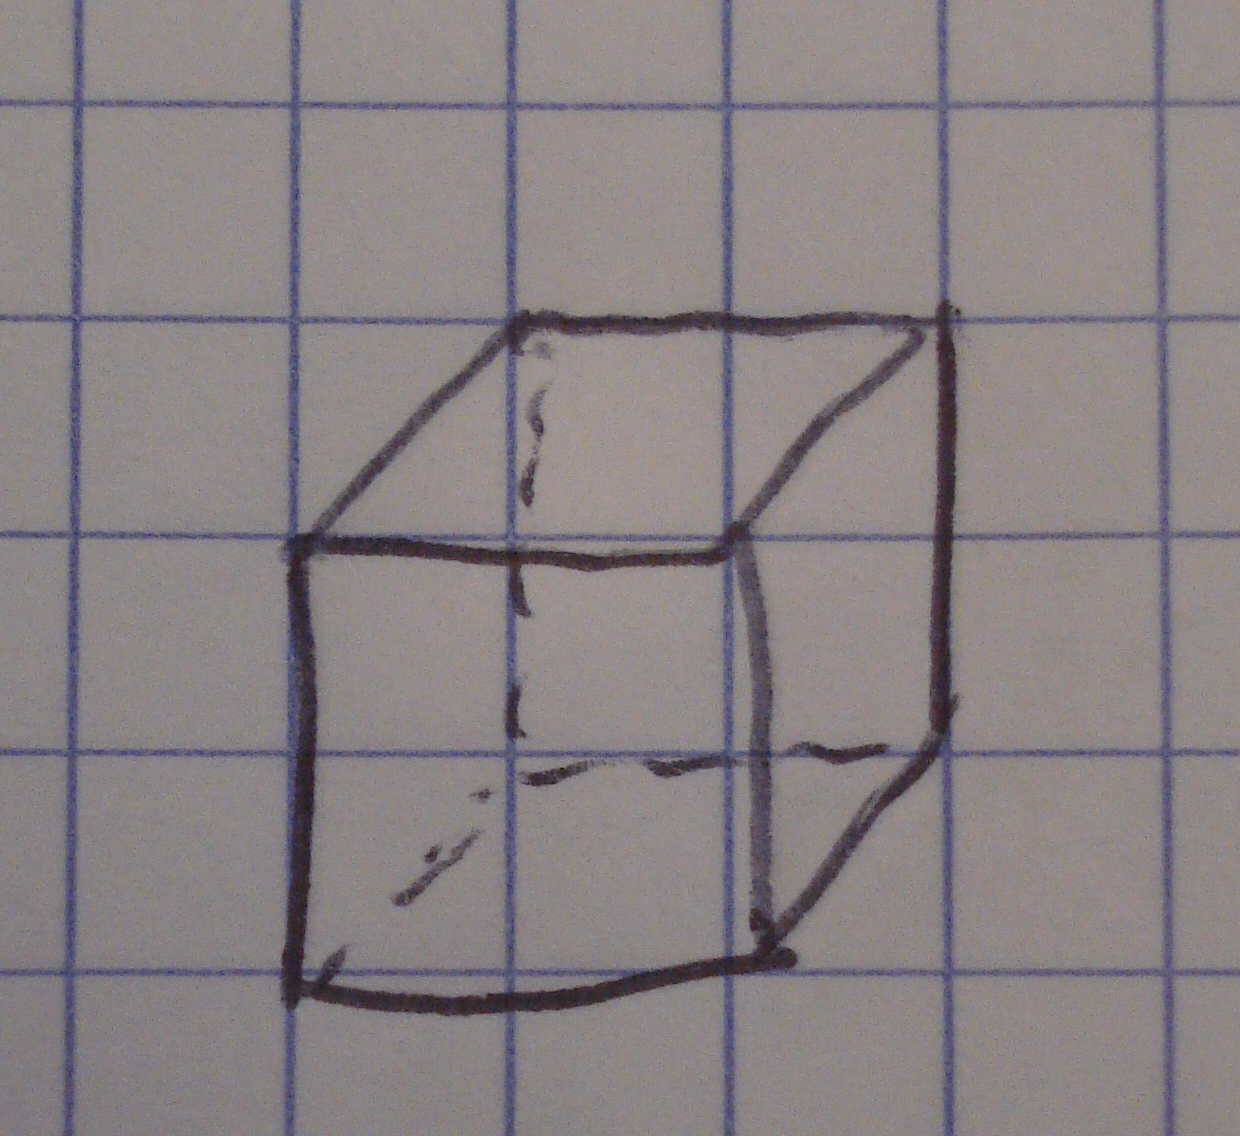
\includegraphics[width=0.6\textwidth]{cube_quadrill.png}
\end{minipage}

\begin{propriete}
    La perspective cavalière respecte les conditions suivantes.
    \begin{enumerate}
        \item
             Deux segments parallèles dans la réalité sont représentés par deux segments parallèles sur le dessin.
         \item
             Trois points alignés dans la réalité sont représentés par trois points alignés sur le dessin.
         \item
             Si \( M\) est le milieu du segment \( [AB]\) dans la réalité, alors \( M\) est le milieu du segment \( [AB]\) dans la réalité.
         \item
             La perspective cavalière respecte les proportions. C'est à dire que si le segment \( [AB]\) est \( p\) fois plus grand que le segment \( [CD]\) dans la réalité, alors il sera \( p\) fois plus grand sur le dessin.
    \end{enumerate}
\end{propriete}

Le cube de la figure \ref{LabelFigCubeLFZuiW} est dessiné avec \( \alpha=\unit{45}{\degree}\) et \( k=0.5\). Notez que les côtés parallèles restent parallèles.
\newcommand{\CaptionFigCubeLFZuiW}{Les segments perpendiculaires à la feuille sont de longueur moitié des autres.}
\input{Fig_CubeLFZuiW.pstricks}

La perspective cavalière n'est pas parfaite; il est aisé de créer des illusions d'optique comme celle de la figure \ref{LabelFigIllusionNHwEtp}. % From file IllusionNHwEtp
\newcommand{\CaptionFigIllusionNHwEtp}{Une petite illusion d'optique facile.}
\input{Fig_IllusionNHwEtp.pstricks}


